\documentclass[aspectratio=169, table, 12pt]{beamer}

\usepackage{colortbl}
\usepackage{xcolor}
\usepackage{listings}
\usepackage{tabularx}
\usepackage{tikz}
\usetikzlibrary{arrows.meta, positioning, calc, fit, shapes.geometric}

\makeatletter
\def\input@path{{../theme/}}
\makeatother
\graphicspath{{../theme/}{../../figures/}}
\usetheme{Pradita}

\definecolor{praditagreen}{RGB}{37, 113, 71}

% Tema membuat garis tabel berwarna putih. Dikembalikan agar tabel terbaca.
\arrayrulecolor{black}
\setlength{\arrayrulewidth}{0.5pt}

% Kolom X rata kiri, dipakai pada tabel dengan kolom X yang sempit, agar
% spasi antarkata tidak meregang.
\newcolumntype{Y}{>{\raggedright\arraybackslash}X}

\lstdefinelanguage{bash}{
  keywords={},
  basicstyle=\ttfamily\scriptsize,
  ndkeywords={cd, curl, docker, python, python3, source},
  ndkeywordstyle=\color{purple}\bfseries,
  sensitive=true,
  commentstyle=\color{gray},
  numbers=none,
  breaklines=true,
  frame=lines,
  backgroundcolor=\color{lightgray!10},
  tabsize=2,
  comment=[l]{\#},
  showstringspaces=false
}

\lstdefinelanguage{TypeScript}{
  keywords={const, let, function, return, async, await, try, catch, throw,
            new, if},
  ndkeywords={Promise, number, fetch, Error},
  basicstyle=\ttfamily\scriptsize,
  keywordstyle=\color{blue}\bfseries,
  ndkeywordstyle=\color{purple}\bfseries,
  sensitive=true,
  commentstyle=\color{gray}\itshape,
  stringstyle=\color{red},
  numbers=none,
  breaklines=true,
  frame=lines,
  backgroundcolor=\color{lightgray!10},
  tabsize=2,
  comment=[l]{//},
  morestring=[b]",
  showstringspaces=false
}

% Gaya Python disamakan dengan naskah bab, tanpa nomor baris.
\lstdefinestyle{PythonStyle}{
  language=Python,
  basicstyle=\ttfamily\scriptsize,
  morekeywords={with, as, yield, async, await, match, case},
  keywordstyle=\color{blue}\bfseries,
  emph={psycopg, ConnectionPool, threading, defaultdict, partial},
  emphstyle=\color{purple}\bfseries,
  commentstyle=\color{gray}\itshape,
  stringstyle=\color{red},
  numbers=none,
  breaklines=true,
  frame=lines,
  backgroundcolor=\color{lightgray!10},
  tabsize=2,
  showstringspaces=false
}

\title{\Huge Caching, Consistency,\\ \vspace{10pt} dan Resilience}
\subtitle{IF140303 - Pengembangan Aplikasi Web}
\author{\textbf{Alfa Yohannis}}

\begin{document}

\frame{\titlepage}

\begin{frame}[fragile]
  \frametitle{Isi Pertemuan}
  \vspace{20pt}
  \begin{columns}[t]
    \column{0.5\textwidth}
    \tableofcontents[sections={1-4}]

    \column{0.5\textwidth}
    \tableofcontents[sections={5-7}]
  \end{columns}
\end{frame}

\begin{frame}{\hfill}
  \centering
  \Huge{\textbf{Kapan salinan boleh dipakai,\\dan berapa lama menunggu?}}
\end{frame}

\section{Tujuan dan Kerangka Bahasan}

\begin{frame}{\hfill}
  \centering
  \Huge{\textbf{Tujuan dan Kerangka Bahasan}}
\end{frame}

\begin{frame}{{\Large Tujuan Pembelajaran}}
  \vspace{12pt}
  \begin{itemize}
    \item Menjelaskan cara browser, Content Delivery Network (CDN), dan
          \textit{cache} aplikasi memutuskan apakah sebuah jawaban boleh
          dipakai ulang, berdasarkan header \texttt{Cache-Control},
          \texttt{ETag}, dan masa berlakunya.
    \item Mengukur untung rugi pola \textit{cache-aside}, termasuk data basi
          dan lonjakan kueri yang muncul ketika sebuah kunci kedaluwarsa.
    \item Merancang batas waktu, \textit{retry}, dan \textit{circuit breaker}
          untuk panggilan ke layanan lain, lalu membuktikan pengaruhnya ketika
          layanan itu melambat.
  \end{itemize}
\end{frame}

\begin{frame}{{\Large Dua Pertanyaan Bab Ini}}
  \vspace{10pt}
  \begin{itemize}
    \item Kueri buku terlaris 30 hari pada Bab 3 tetap memakan puluhan
          milidetik walaupun indeksnya sudah dipasang.
    \item Jawabannya sama untuk semua pengunjung, dan hanya berubah sedikit
          dari menit ke menit.
    \item \textit{Caching} menyimpan jawaban yang sudah jadi, lalu memakainya
          lagi. Harganya: salinan dapat basi, dan tempat penyimpanannya dapat
          lambat atau mati.
  \end{itemize}
  \vspace{8pt}
  {\footnotesize Dua pertanyaan: kapan sebuah salinan boleh dipakai, dan apa
  yang terjadi ketika komponen yang dipanggil aplikasi bermasalah.}
\end{frame}

\section{Caching di Browser dan HTTP}

\begin{frame}{\hfill}
  \centering
  \Huge{\textbf{Caching di Browser\\dan HTTP}}
\end{frame}

\begin{frame}{{\Large Segar atau Basi}}
  \vspace{10pt}
  \begin{itemize}
    \item Salinan yang masih segar langsung dipakai, tanpa menghubungi server
          sama sekali.
    \item Salinan yang basi ditanyakan ulang. Browser mengirim tanda versi
          salinannya lewat \texttt{If-None-Match}, berisi nilai \texttt{ETag}
          dari server.
    \item Server menjawab \texttt{304 Not Modified} tanpa isi bila belum
          berubah, atau \texttt{200} dengan isi baru bila sudah berubah.
  \end{itemize}
  \vspace{8pt}
  {\footnotesize Analoginya fotokopi jadwal ujian bertuliskan ``berlaku sampai
  Jumat'' dan ``versi 7''. Setelah Jumat, mahasiswa cukup bertanya ``versi 7
  masih berlaku?'', dan petugas cukup menjawab ``masih''.}
\end{frame}

\begin{frame}{{\Large Keputusan Browser}}
  \vspace{4pt}
  \centering
  \scalebox{1.05}{
  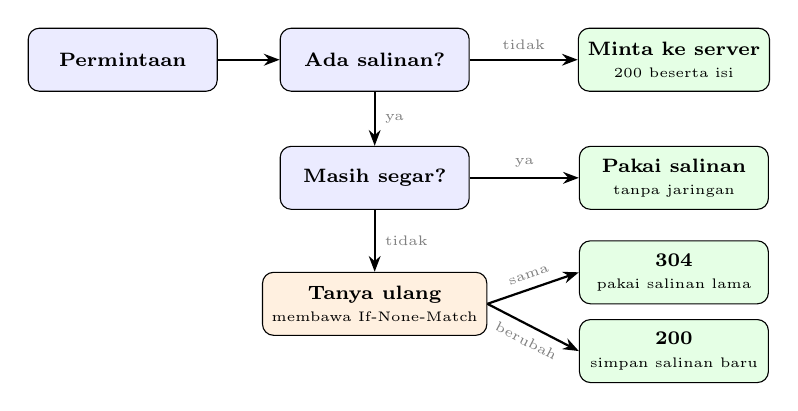
\begin{tikzpicture}[
    font=\scriptsize,
    kotak/.style={draw, rounded corners, align=center, minimum height=0.8cm,
                  minimum width=2.4cm, fill=blue!8, font=\scriptsize\bfseries},
    hasil/.style={kotak, fill=green!10},
    panah/.style={-{Stealth[length=2mm]}, thick},
    ket/.style={font=\tiny, gray}
  ]
    \node[kotak] (minta) at (0,0) {Permintaan};
    \node[kotak] (ada) at (3.2,0) {Ada salinan?};
    \node[hasil] (ambil) at (7.0,0)
      {Minta ke server\\{\tiny\mdseries 200 beserta isi}};
    \node[kotak] (segar) at (3.2,-1.5) {Masih segar?};
    \node[hasil] (pakai) at (7.0,-1.5)
      {Pakai salinan\\{\tiny\mdseries tanpa jaringan}};
    \node[kotak, fill=orange!12] (tanya) at (3.2,-3.1)
      {Tanya ulang\\{\tiny\mdseries membawa If-None-Match}};
    \node[hasil] (tetap) at (7.0,-2.7)
      {304\\{\tiny\mdseries pakai salinan lama}};
    \node[hasil] (baru) at (7.0,-3.7)
      {200\\{\tiny\mdseries simpan salinan baru}};
    \draw[panah] (minta) -- (ada);
    \draw[panah] (ada) -- node[ket, above] {tidak} (ambil);
    \draw[panah] (ada) -- node[ket, right] {ya} (segar);
    \draw[panah] (segar) -- node[ket, above] {ya} (pakai);
    \draw[panah] (segar) -- node[ket, right] {tidak} (tanya);
    \draw[panah] (tanya.east) -- node[ket, above, sloped] {sama} (tetap.west);
    \draw[panah] (tanya.east) -- node[ket, below, sloped] {berubah} (baru.west);
  \end{tikzpicture}}
\end{frame}

\begin{frame}{{\Large Perintah Cache-Control}}
  \vspace{6pt}
  \centering
  {\footnotesize
  \begin{tabularx}{\textwidth}{lX}
    \hline
    \textbf{Perintah} & \textbf{Artinya} \\
    \hline
    \texttt{max-age=N} & Salinan segar selama N detik sejak jawaban dibuat. Selama itu server tidak ditanya. \\
    \hline
    \texttt{s-maxage=N} & Sama dengan \texttt{max-age}, tetapi khusus untuk \textit{cache} bersama seperti CDN. Browser mengabaikannya. \\
    \hline
    \texttt{no-cache} & Salinan boleh disimpan, tetapi setiap pemakaian wajib ditanyakan ulang ke server. \\
    \hline
    \texttt{no-store} & Jawaban tidak boleh disimpan sama sekali, di mana pun. \\
    \hline
    \texttt{private} & Hanya browser pengguna itu yang boleh menyimpan. CDN dan \textit{proxy} tidak boleh. \\
    \hline
  \end{tabularx}}
\end{frame}

\begin{frame}{{\Large Perintah Cache-Control (Lanjutan)}}
  \vspace{6pt}
  \centering
  {\footnotesize
  \begin{tabularx}{\textwidth}{lX}
    \hline
    \textbf{Perintah} & \textbf{Artinya} \\
    \hline
    \texttt{public} & \textit{Cache} bersama boleh menyimpan, walaupun permintaannya membawa header \texttt{Authorization}. \\
    \hline
    \texttt{immutable} & Isinya tidak berubah selama masih segar, sehingga memuat ulang halaman pun tidak memicu pertanyaan ulang. \\
    \hline
    \texttt{stale-while-revalidate=N} & Setelah basi, salinan masih boleh dipakai selama N detik sambil diperbarui di belakang layar. \\
    \hline
    \texttt{stale-if-error=N} & Setelah basi, salinan masih boleh dipakai selama N detik bila server sedang \textit{error}. \\
    \hline
  \end{tabularx}}
\end{frame}

\begin{frame}{{\Large no-cache dan no-store Sering Tertukar}}
  \vspace{10pt}
  \begin{itemize}
    \item \texttt{no-cache} membolehkan jawaban disimpan, tetapi setiap
          pemakaiannya harus ditanyakan ulang ke server.
    \item \texttt{no-store} melarang jawaban disimpan sama sekali.
    \item Halaman yang diberi \texttt{no-cache} tetap tersimpan di browser.
          Untuk halaman yang tidak boleh tertinggal di komputer pengguna,
          misalnya halaman rekening, dipakai \texttt{no-store}.
  \end{itemize}
\end{frame}

\begin{frame}{{\Large Dua Contoh dari Aplikasi}}
  \vspace{8pt}
  \begin{enumerate}
    \item \texttt{app.3f9a2c.js} dikirim dengan \texttt{max-age=31536000},
          yaitu satu tahun, ditambah \texttt{immutable}. Ketika isinya
          berubah, namanya ikut berubah, misalnya menjadi
          \texttt{app.9b1e07.js}.
    \item Halaman HyperText Markup Language (HTML) dikirim dengan
          \texttt{no-cache} dan \texttt{ETag}. Permintaan pertama menerima 331
          byte. Permintaan bersyarat menerima status 304 dengan 0 byte.
  \end{enumerate}
  \vspace{8pt}
  {\footnotesize Jawaban 304 menghemat isi, tetapi browser tetap menunggu satu
  \textit{round-trip time} (RTT) untuk mendapatkannya.}
\end{frame}

\begin{frame}[fragile]{{\Large Memilih antara 200 dan 304}}
  \vspace{2pt}
\begin{lstlisting}[style=PythonStyle]
  def layani_halaman(self, sertakan_isi):
    """Menjawab 304 bila ETag kiriman browser masih sama, 200 bila tidak."""
    header_tambahan = {
        "Cache-Control": CACHE_CONTROL_HALAMAN,
        "ETag": self.server.etag_halaman,
    }
    if self.headers.get("If-None-Match") == self.server.etag_halaman:
      # 304 tidak membawa isi. Browser memakai salinan yang sudah dimilikinya.
      self.kirim_jawaban(304, b"", "text/html", header_tambahan,
                         sertakan_isi=False)
      return
    jenis_isi = "text/html; charset=utf-8"
    self.kirim_jawaban(200, self.server.isi_halaman, jenis_isi,
                       header_tambahan, sertakan_isi)
\end{lstlisting}

  \vspace{2pt}
  {\footnotesize Server cukup membandingkan \texttt{ETag} miliknya dengan nilai
  \texttt{If-None-Match} kiriman browser.}
\end{frame}

\begin{frame}[fragile]{{\Large Validasi Ulang dengan curl}}
  \vspace{4pt}
\begin{lstlisting}[language=bash]
curl -sI http://localhost:8000/ | grep -iE "^(http|cache-control|etag)"
curl -s -o /dev/null -w "%{http_code} %{size_download} byte\n" \
  -H 'If-None-Match: "7f63aec6090e2c3f"' http://localhost:8000/

# Keluarannya:
# HTTP/1.0 200 OK
# Cache-Control: no-cache
# ETag: "7f63aec6090e2c3f"
# 304 0 byte
\end{lstlisting}

  \vspace{4pt}
  {\footnotesize Nilai \texttt{ETag} dari perintah pertama dipakai sebagai isi
  \texttt{If-None-Match} pada perintah kedua.}
\end{frame}

\begin{frame}{{\Large Bila Server Tidak Menulis Kebijakan}}
  \vspace{10pt}
  \begin{itemize}
    \item Aset \texttt{stylenew.css} situs kampus hanya mengirim
          \texttt{Last-Modified} dan \texttt{ETag}.
    \item Request for Comments (RFC) 9111 membolehkan browser menebak masa
          segar dari umur berkas. Angka yang lazim adalah sepersepuluh selang
          sejak berkas terakhir diubah.
    \item Berkas diubah 14 Maret 2025. Pada 10 September 2026 umurnya sekitar
          545 hari, sehingga dianggap segar sekitar 54 hari.
  \end{itemize}
  \vspace{8pt}
  {\footnotesize Itulah sebab aset yang tercatat 0 milidetik pada Latihan 2 di
  Bab 2.}
\end{frame}

\begin{frame}{{\Large Kebijakan Menurut Jenis Sumber}}
  \vspace{4pt}
  \centering
  {\scriptsize
  \begin{tabularx}{\textwidth}{lYY}
    \hline
    \textbf{Jenis sumber} & \textbf{\texttt{Cache-Control}} & \textbf{Alasannya} \\
    \hline
    \textit{Fingerprinted asset} & \texttt{public, max-age=31536000, immutable} & Isinya tidak pernah berubah tanpa namanya ikut berubah. \\
    \hline
    Halaman HTML & \texttt{no-cache}, disertai \texttt{ETag} & Alamatnya tetap, sehingga perubahan hanya ketahuan lewat pertanyaan ulang. \\
    \hline
    Data umum dari API & \texttt{public, s-maxage=60, stale-while-revalidate=30} & CDN menyimpannya sebentar, dan sedikit basi masih dapat diterima. \\
    \hline
    Data pribadi pengguna & \texttt{private, no-cache} & Tidak boleh tersimpan di \textit{cache} bersama. \\
    \hline
    Data rahasia & \texttt{no-store} & Tidak boleh tertinggal di mana pun, termasuk di cakram pengguna. \\
    \hline
  \end{tabularx}}

  \vspace{6pt}
  {\footnotesize API adalah singkatan dari Application Programming Interface.}
\end{frame}

\section{CDN dan Cache Tingkat Aplikasi}

\begin{frame}{\hfill}
  \centering
  \Huge{\textbf{CDN dan Cache\\Tingkat Aplikasi}}
\end{frame}

\begin{frame}{{\Large Makin Dekat ke Pengguna}}
  \vspace{4pt}
  \centering
  \scalebox{0.95}{
  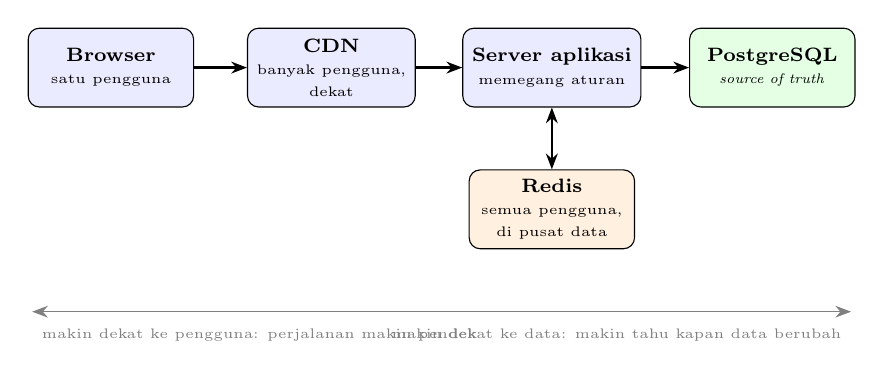
\begin{tikzpicture}[
    font=\scriptsize,
    lapisan/.style={draw, rounded corners, align=center, minimum height=1.0cm,
                    minimum width=2.1cm, fill=blue!8, font=\scriptsize\bfseries},
    panah/.style={-{Stealth[length=2mm]}, thick}
  ]
    \node[lapisan] (browser) at (0,0) {Browser\\{\tiny\mdseries satu pengguna}};
    \node[lapisan] (cdn) at (2.8,0)
      {CDN\\{\tiny\mdseries banyak pengguna,}\\{\tiny\mdseries dekat}};
    \node[lapisan] (aplikasi) at (5.6,0)
      {Server aplikasi\\{\tiny\mdseries memegang aturan}};
    \node[lapisan, fill=green!10] (db) at (8.4,0)
      {PostgreSQL\\{\tiny\mdseries \textit{source of truth}}};
    \node[lapisan, fill=orange!12] (redis) at (5.6,-1.8)
      {Redis\\{\tiny\mdseries semua pengguna,}\\{\tiny\mdseries di pusat data}};
    \draw[panah] (browser) -- (cdn);
    \draw[panah] (cdn) -- (aplikasi);
    \draw[panah] (aplikasi) -- (db);
    \draw[{Stealth[length=2mm]}-{Stealth[length=2mm]}, thick]
      (aplikasi) -- (redis);
    \draw[{Stealth[length=2mm]}-{Stealth[length=2mm]}, gray]
      (-1.0,-3.1) -- (9.4,-3.1);
    \node[font=\tiny, gray, anchor=north west] at (-1.0,-3.2)
      {makin dekat ke pengguna: perjalanan makin pendek};
    \node[font=\tiny, gray, anchor=north east] at (9.4,-3.2)
      {makin dekat ke data: makin tahu kapan data berubah};
  \end{tikzpicture}}

  \vspace{4pt}
  {\footnotesize Analoginya toko buku dengan gudang cabang. Gudang cabang cepat
  dijangkau, tetapi tidak tahu kapan penerbit menaikkan harga. Gudang pusat
  tahu semuanya, tetapi letaknya jauh.}
\end{frame}

\begin{frame}{{\Large Perbandingan Titik Penyimpanan}}
  \vspace{4pt}
  \centering
  {\scriptsize
  \begin{tabularx}{\textwidth}{lYYY}
    \hline
    \textbf{Titik} & \textbf{Dipakai oleh} & \textbf{Diatur lewat} & \textbf{Cara membuang salinan} \\
    \hline
    Browser & Satu pengguna & Header \texttt{Cache-Control} dari server & Tidak dapat dari server. Tunggu kedaluwarsa, atau ganti nama berkas. \\
    \hline
    CDN & Banyak pengguna di satu wilayah & \texttt{Cache-Control}, terutama \texttt{s-maxage}, dan aturan di panel CDN & Perintah \textit{purge} ke penyedia CDN. \\
    \hline
    Redis & Seluruh pengguna aplikasi & Kode aplikasi & Menghapus kunci dari kode, tepat setelah data diubah. \\
    \hline
    Memori basis data & Seluruh kueri & Basis data sendiri, lewat \texttt{shared\_buffers} & Otomatis, tidak perlu diatur. \\
    \hline
  \end{tabularx}}

  \vspace{6pt}
  {\footnotesize Kolom terakhir menentukan berapa lama sebuah kesalahan
  bertahan.}
\end{frame}

\begin{frame}{{\Large CDN Adalah Cache Bersama}}
  \vspace{8pt}
  \begin{enumerate}
    \item Halaman katalog umum dengan \texttt{s-maxage=60}: tiap server CDN
          bertanya ke server \textit{origin} paling banyak sekali per 60 detik. Dengan 20
          server CDN, server \textit{origin} menerima paling banyak 20 permintaan per
          menit, walaupun pengunjungnya 10.000 orang.
    \item Halaman yang memuat nama pengguna keliru diberi \texttt{public}.
          Salinan milik pengguna pertama terkirim ke pengguna berikutnya.
          Halaman semacam itu diberi \texttt{private}.
  \end{enumerate}
  \vspace{6pt}
  {\footnotesize \texttt{Vary: Accept-Encoding} wajar. \texttt{Vary: Cookie}
  membuat tiap pengguna punya salinan sendiri, sehingga CDN hampir tidak pernah
  menemukan salinan yang dapat dipakai ulang.}
\end{frame}

\begin{frame}{{\Large Kapan Hasil Kueri Layak Disimpan}}
  \vspace{10pt}
  \begin{itemize}
    \item Tiga syaratnya: mahal dihitung, dibaca jauh lebih sering daripada
          berubah, dan boleh sedikit basi.
    \item Buku terlaris 30 hari memenuhi ketiganya: sekitar 70 milidetik, sama
          untuk semua pengunjung, dan hampir tidak bergeser dalam satu menit.
    \item Q1 pada Bab 3 hanya memakan 0,016 milidetik di dalam basis data.
          Menyimpannya di Redis tidak menghemat apa pun yang berarti, tetapi
          menambah kemungkinan data basi.
  \end{itemize}
\end{frame}

\section{Pola Cache-Aside dengan Redis}

\begin{frame}{\hfill}
  \centering
  \Huge{\textbf{Pola Cache-Aside\\dengan Redis}}
\end{frame}

\begin{frame}{{\Large Pola Cache-Aside}}
  \vspace{8pt}
  \begin{itemize}
    \item Membaca: periksa Redis. Bila ada (HIT), langsung dipakai. Bila tidak
          ada (MISS), baca basis data, simpan ke Redis beserta \textit{Time To
          Live} (TTL), lalu dipakai.
    \item Menulis: ubah basis data lebih dahulu, lalu hapus kunci terkait di
          Redis.
    \item Redis tidak pernah menjadi \textit{source of truth}. Bila Redis kosong atau
          mati, jawaban tetap benar, hanya lebih lambat.
  \end{itemize}
  \vspace{6pt}
  {\footnotesize Analoginya warung dengan kulkas di depan. Bila kulkas kosong,
  penjual mengambil dari gudang belakang sekalian mengisi kulkas. Kulkas boleh
  kosong kapan saja, dan warung tetap berjualan.}
\end{frame}

\begin{frame}{{\Large Urutan Pesan: Satu MISS, Lalu Satu HIT}}
  \vspace{2pt}
  \centering
  \scalebox{0.85}{
  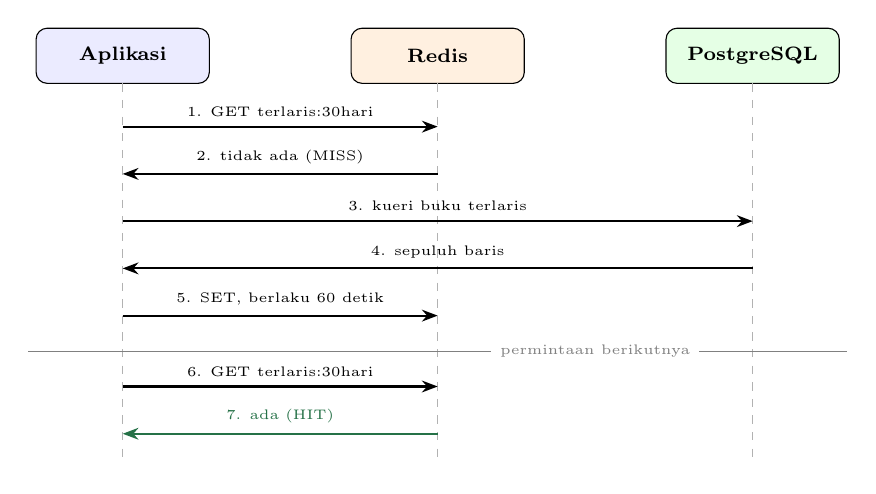
\begin{tikzpicture}[
    font=\scriptsize,
    kepala/.style={draw, rounded corners, align=center, minimum height=0.7cm,
                   minimum width=2.2cm, fill=blue!8, font=\scriptsize\bfseries},
    panah/.style={-{Stealth[length=2mm]}, thick},
    garis/.style={gray!60, dashed},
    pesan/.style={font=\tiny, above, midway}
  ]
    \node[kepala] at (0,0) {Aplikasi};
    \node[kepala, fill=orange!12] at (4,0) {Redis};
    \node[kepala, fill=green!10] at (8,0) {PostgreSQL};
    \foreach \x in {0,4,8} \draw[garis] (\x,-0.35) -- (\x,-5.2);
    \draw[panah] (0,-0.9) -- node[pesan] {1. GET terlaris:30hari} (4,-0.9);
    \draw[panah] (4,-1.5) -- node[pesan] {2. tidak ada (MISS)} (0,-1.5);
    \draw[panah] (0,-2.1) -- node[pesan] {3. kueri buku terlaris} (8,-2.1);
    \draw[panah] (8,-2.7) -- node[pesan] {4. sepuluh baris} (0,-2.7);
    \draw[panah] (0,-3.3) -- node[pesan] {5. SET, berlaku 60 detik} (4,-3.3);
    \draw[gray, thin] (-1.2,-3.75) -- (9.2,-3.75);
    \node[fill=white, font=\tiny, text=gray] at (6,-3.75) {permintaan berikutnya};
    \draw[panah] (0,-4.2) -- node[pesan] {6. GET terlaris:30hari} (4,-4.2);
    \draw[panah, praditagreen] (4,-4.8) -- node[pesan] {7. ada (HIT)} (0,-4.8);
  \end{tikzpicture}}

  {\footnotesize Basis data hanya disentuh ketika kunci tidak ditemukan.}
\end{frame}

\begin{frame}[fragile]{{\Large Membaca dari Cache}}
  \vspace{4pt}
\begin{lstlisting}[style=PythonStyle]
def baca_dari_cache(cache, kunci):
  """Membaca satu kunci dari Redis, atau None bila kuncinya tidak ada.

  Error Redis sengaja ditelan. Cache bukan source of truth, sehingga Redis
  yang mati hanya membuat aplikasi lebih lambat, bukan ikut mati.
  """
  try:
    return cache.get(kunci)
  except redis.RedisError:
    return None
\end{lstlisting}

  \vspace{4pt}
  {\footnotesize Redis yang bermasalah diperlakukan sama dengan kunci yang
  tidak ada.}
\end{frame}

\begin{frame}[fragile]{{\Large Cache-Aside dalam Kode}}
  \vspace{4pt}
\begin{lstlisting}[style=PythonStyle]
def ambil_terlaris_lewat_cache(pool_koneksi, cache):
  """Pola cache-aside: periksa cache, bila tidak ada hitung lalu simpan.

  Mengembalikan pasangan (isi JSON dalam bentuk byte, "HIT" atau "MISS").
  """
  isi_tersimpan = baca_dari_cache(cache, KUNCI_TERLARIS)
  if isi_tersimpan is not None:
    return isi_tersimpan, "HIT"
  isi_json = json.dumps(jalankan_kueri_terlaris(pool_koneksi)).encode()
  simpan_ke_cache(cache, KUNCI_TERLARIS, isi_json, TTL_TERLARIS_DETIK)
  return isi_json, "MISS"
\end{lstlisting}

  \vspace{4pt}
  {\footnotesize Tersedia di \texttt{sources/chapter04/aplikasi.py}.}
\end{frame}

\begin{frame}{{\Large Hasil Pengukuran}}
  \vspace{4pt}
  \centering
  {\footnotesize
  \begin{tabularx}{\textwidth}{Xrrrl}
    \hline
    \textbf{Keadaan} & \textbf{p50} & \textbf{p95} & \textbf{Terbesar} & \textbf{Asal jawaban} \\
    \hline
    Tanpa \textit{cache}, 50 permintaan & 70,44 & 81,99 & 94,41 & 50 kueri ke basis data \\
    \hline
    \textit{Cache-aside}, 50 permintaan & 0,31 & 0,63 & 67,55 & 1 MISS, 49 HIT \\
    \hline
    Redis dibekukan, 20 permintaan & 184,72 & 188,85 & 189,07 & 20 MISS \\
    \hline
  \end{tabularx}}

  \vspace{6pt}
  \begin{itemize}
    \item Waktu sampai byte pertama dalam milidetik, diukur dengan cara yang
          sama dengan kolom \texttt{TungguServer} pada Bab 2.
    \item p50 turun dari 70,44 menjadi 0,31 milidetik, sekitar 227 kali lebih
          cepat. Nilai terbesar 67,55 milidetik adalah satu-satunya MISS.
  \end{itemize}
\end{frame}

\begin{frame}{{\Large Cache yang Macet}}
  \vspace{8pt}
  \begin{itemize}
    \item Redis dibekukan dengan \texttt{docker compose pause}, sehingga tidak
          menjawab perintah apa pun.
    \item Tiap permintaan menunggu 50 milidetik untuk GET, menjalankan kueri,
          lalu menunggu 50 milidetik lagi untuk SET: 184,72 milidetik.
    \item Hasilnya lebih dari dua kali lipat keadaan tanpa \textit{cache}.
          \textit{Cache} yang macet lebih buruk daripada tidak ada
          \textit{cache} sama sekali.
  \end{itemize}
  \vspace{6pt}
  {\footnotesize Aplikasi tetap menjawab karena \textit{error} Redis ditelan dan setiap
  perintah Redis dibatasi 50 milidetik, setelah \textit{retry} bawaan pustakanya
  dimatikan.}
\end{frame}

\begin{frame}{{\Large Dua Konsekuensi dan Satu Peringatan}}
  \vspace{8pt}
  \begin{enumerate}
    \item Kegagalan \textit{cache} tidak boleh menjatuhkan aplikasi. Setiap
          \textit{error} Redis diteruskan menjadi pembacaan ke basis data.
    \item Setiap panggilan ke \textit{cache} membutuhkan batas waktu yang jauh
          lebih kecil daripada kueri yang ingin dihindarinya.
  \end{enumerate}
  \vspace{6pt}
  {\footnotesize Redis pada bab ini dibatasi 64 MB dengan kebijakan
  \texttt{allkeys-lru}. Ketika penuh, kunci yang paling lama tidak dipakai
  dibuang, atau \textit{Least Recently Used} (LRU). Kunci yang pernah disimpan
  belum tentu masih ada.}
\end{frame}

\section{Invalidasi, TTL, dan Stale-While-Revalidate}

\begin{frame}{\hfill}
  \centering
  \Huge{\textbf{Invalidasi, TTL, dan\\Stale-While-Revalidate}}
\end{frame}

\begin{frame}{{\Large TTL dan Invalidasi}}
  \vspace{10pt}
  \begin{itemize}
    \item Salinan menjadi basi ketika data aslinya berubah.
    \item TTL: salinan kedaluwarsa sendiri setelah sekian detik.
    \item Invalidasi: kode yang mengubah data langsung menghapus salinannya,
          sehingga pembacaan berikutnya terpaksa mengambil data baru.
  \end{itemize}
  \vspace{8pt}
  {\footnotesize Analoginya papan harga di warung. Papan yang diperbarui tiap
  pagi baru menampilkan kenaikan harga besok pagi. Pemilik yang menghapus harga
  begitu harga naik memaksa pembeli berikutnya bertanya ke kasir.}
\end{frame}

\begin{frame}{{\Large Cara Membatasi Data Basi}}
  \vspace{4pt}
  \centering
  {\scriptsize
  \begin{tabularx}{\textwidth}{lYY}
    \hline
    \textbf{Cara} & \textbf{Cara kerjanya} & \textbf{Kelemahannya} \\
    \hline
    TTL saja & Salinan dibiarkan sampai masa berlakunya habis. & Data basi selama sisa TTL, paling lama sepanjang TTL itu sendiri. \\
    \hline
    Hapus saat menulis & Kunci dihapus tepat setelah basis data diubah. & Dapat kalah dalam \textit{race condition} dengan pembaca yang lambat. \\
    \hline
    Hapus dua kali & Kunci dihapus sekali lagi beberapa saat kemudian, disebut \textit{delayed double delete}. & Masih ada jendela basi sepanjang jeda penghapusan kedua. \\
    \hline
    Kunci berversi & Nomor versi menjadi bagian nama kunci, misalnya \texttt{buku:1:v8}. & Pembaca harus tahu nomor versi terbaru lebih dahulu, dan kunci versi lama tertinggal sampai TTL-nya habis. \\
    \hline
  \end{tabularx}}
\end{frame}

\begin{frame}{{\Large Race Condition Saat Menghapus}}
  \vspace{4pt}
  \centering
  {\small
  \begin{tabularx}{\textwidth}{lXXll}
    \hline
    \textbf{Waktu} & \textbf{Pembaca} & \textbf{Penulis} & \textbf{\textit{Cache}} & \textbf{Basis data} \\
    \hline
    t1 & \texttt{GET} $\rightarrow$ tidak ada & & kosong & 50.000 \\
    \hline
    t2 & \texttt{SELECT} $\rightarrow$ 50.000 & & kosong & 50.000 \\
    \hline
    t3 & & \texttt{UPDATE} $\rightarrow$ 55.000 & kosong & 55.000 \\
    \hline
    t4 & & \texttt{DEL} & kosong & 55.000 \\
    \hline
    t5 & \texttt{SET} 50.000 & & 50.000 & 55.000 \\
    \hline
  \end{tabularx}}

  \vspace{8pt}
  {\footnotesize Penghapusan pada t4 tidak menghapus apa pun, karena kuncinya
  belum ada. Harga lama yang disimpan pada t5 bertahan sampai TTL habis, dan
  tidak ada \textit{error} yang muncul.}
\end{frame}

\begin{frame}{{\Large Lama Harga Lama Masih Terbaca}}
  \vspace{4pt}
  \centering
  {\small
  \begin{tabularx}{\textwidth}{Xrr}
    \hline
    \textbf{Cara} & \textbf{Pembacaan basi} & \textbf{Lama basi (detik)} \\
    \hline
    \texttt{ttl\_saja} & 50 & 5,1 \\
    \hline
    \texttt{hapus\_saat\_menulis} & 0 & 0,0 \\
    \hline
    \texttt{hapus\_kalah\_race} & 50 & 5,1 \\
    \hline
    \texttt{hapus\_dua\_kali} & 5 & 0,5 \\
    \hline
  \end{tabularx}}

  \vspace{6pt}
  \begin{itemize}
    \item Harga diubah dari 50.000 menjadi 55.000, TTL 5 detik, dibaca setiap
          100 milidetik.
    \item Penghapusan yang kalah dalam \textit{race condition} sama buruknya dengan tanpa
          penghapusan. Kelebihan 0,1 detik berasal dari selang pemeriksaan.
  \end{itemize}
\end{frame}

\begin{frame}[fragile]{{\Large Penghapusan Kedua}}
  \vspace{4pt}
\begin{lstlisting}[style=PythonStyle]
  sudah_membaca.wait()
  ubah_harga_di_basis_data(koneksi, HARGA_BARU)
  cache.delete(KUNCI_HARGA)
  if hapus_sekali_lagi:
    # Penghapusan kedua menyapu harga lama yang sempat diisi ulang pembaca.
    threading.Timer(
        JEDA_HAPUS_KEDUA_DETIK, cache.delete, args=(KUNCI_HARGA,)
    ).start()
\end{lstlisting}

  \vspace{4pt}
  {\footnotesize Jendela basi menyusut menjadi 0,5 detik. Cara yang lebih rapi
  dipakai Facebook: \textit{cache} memberi token (\textit{lease}) saat kunci
  tidak ditemukan, penghapusan membatalkan token itu, dan penyimpanan dengan
  token batal ditolak.}
\end{frame}

\begin{frame}{{\Large Berapa Panjang TTL}}
  \vspace{8pt}
  Ukurannya: berapa lama pengguna boleh melihat data lama tanpa dirugikan.
  \vspace{4pt}
  \begin{enumerate}
    \item Daftar buku terlaris diberi TTL 60 detik. Selisih satu menit tidak
          merugikan siapa pun.
    \item Harga dan stok pada saat pembayaran tidak dibaca dari
          \textit{cache} sama sekali. Harga yang basi 5 detik saja dapat
          membuat pembeli membayar harga lama.
  \end{enumerate}
  \vspace{6pt}
  {\footnotesize Kunci dengan TTL sama yang disimpan bersamaan akan kedaluwarsa
  bersamaan. TTL diberi tambahan acak kecil, misalnya 60 detik ditambah acak 0
  sampai 6 detik.}
\end{frame}

\begin{frame}{{\Large Cache Stampede}}
  \vspace{10pt}
  \begin{itemize}
    \item Kunci yang sering dibaca kedaluwarsa, lalu banyak permintaan meleset
          pada saat yang sama dan menjalankan kueri yang sama.
    \item \texttt{stampede.py} melepas 50 permintaan serentak dengan
          \textit{pool} berisi 10 koneksi, pada tiga cara:
          \texttt{tanpa\_pengaman}, \texttt{single\_flight}, dan
          \texttt{stale\_while\_revalidate}.
  \end{itemize}
  \vspace{8pt}
  {\footnotesize Analoginya warung yang kulkasnya mendadak kosong saat jam
  istirahat: sepuluh pembeli sekaligus pergi ke gudang belakang untuk
  mengambil minuman yang sama.}
\end{frame}

\begin{frame}{{\Large Hasil: 50 Permintaan Serentak}}
  \vspace{4pt}
  \centering
  {\small
  \begin{tabularx}{\textwidth}{Xrrrr}
    \hline
    \textbf{Cara} & \textbf{Kueri} & \textbf{p50} & \textbf{p95} & \textbf{Terbesar} \\
    \hline
    \texttt{tanpa\_pengaman} & 50 & 895,7 & 1.529,3 & 1.564,3 \\
    \hline
    \texttt{single\_flight} & 1 & 137,5 & 143,2 & 143,7 \\
    \hline
    \texttt{stale\_while\_revalidate} & 1 & 8,8 & 12,6 & 14,0 \\
    \hline
  \end{tabularx}}

  \vspace{6pt}
  \begin{itemize}
    \item Tanpa pengaman, 50 kueri mengantre dalam lima gelombang: p50-nya
          hampir tujuh kali lipat satu kueri yang berjalan sendirian, yaitu
          135,2 milidetik.
    \item Dengan \textit{single-flight}, hanya satu kueri yang sampai ke basis
          data.
  \end{itemize}
\end{frame}

\begin{frame}[fragile]{{\Large Single-Flight: Satu Menghitung}}
  \vspace{2pt}
\begin{lstlisting}[style=PythonStyle]
def single_flight(pool_koneksi, cache, penghitung_kueri):
  """Hanya pemegang gembok yang menghitung, sisanya menunggu hasilnya muncul.

  SET NX berhasil bagi tepat satu klien. Klien lain memeriksa ulang cache
  setiap 10 milidetik sampai nilainya tersedia.
  """
  nilai_tersimpan = cache.get(KUNCI_TERLARIS)
  if nilai_tersimpan is not None:
    return nilai_tersimpan
  if cache.set(KUNCI_GEMBOK, "1", nx=True, px=UMUR_GEMBOK_MS):
    isi_json = jalankan_kueri_terlaris(pool_koneksi, penghitung_kueri)
    cache.set(KUNCI_TERLARIS, isi_json, ex=TTL_KERAS_DETIK)
    cache.delete(KUNCI_GEMBOK)
    return isi_json
\end{lstlisting}
\end{frame}

\begin{frame}[fragile]{{\Large Single-Flight: Sisanya Menunggu}}
  \vspace{4pt}
\begin{lstlisting}[style=PythonStyle]
  batas_waktu_tunggu = time.monotonic() + BATAS_MENUNGGU_DETIK
  while time.monotonic() < batas_waktu_tunggu:
    time.sleep(JEDA_PERIKSA_ULANG_DETIK)
    nilai_tersimpan = cache.get(KUNCI_TERLARIS)
    if nilai_tersimpan is not None:
      return nilai_tersimpan
  # Pemegang gembok terlalu lama, jadi hitung sendiri daripada gagal.
  return jalankan_kueri_terlaris(pool_koneksi, penghitung_kueri)
\end{lstlisting}

  \vspace{4pt}
  {\footnotesize Perintah \texttt{SET} dengan \texttt{nx=True} hanya berhasil
  bila kuncinya belum ada, sehingga tepat satu klien memperoleh gembok.
  Tersedia di \texttt{sources/chapter04/stampede.py}.}
\end{frame}

\begin{frame}{{\Large Dua Batas Waktu}}
  \vspace{10pt}
  \centering
  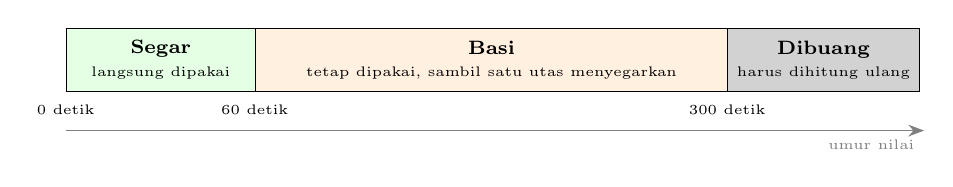
\begin{tikzpicture}[
    font=\scriptsize,
    pita/.style={draw, minimum height=0.8cm, anchor=west, align=center,
                 font=\scriptsize\bfseries}
  ]
    \node[pita, fill=green!10, minimum width=2.4cm] at (0,0)
      {Segar\\{\tiny\mdseries langsung dipakai}};
    \node[pita, fill=orange!12, minimum width=6.0cm] at (2.4,0)
      {Basi\\{\tiny\mdseries tetap dipakai, sambil satu utas menyegarkan}};
    \node[pita, fill=gray!35, minimum width=2.4cm] at (8.4,0)
      {Dibuang\\{\tiny\mdseries harus dihitung ulang}};
    \foreach \x/\teks in {0/0 detik, 2.4/60 detik, 8.4/300 detik}
      \node[font=\tiny, anchor=north] at (\x,-0.45) {\teks};
    \draw[-{Stealth[length=2mm]}, gray] (0,-0.9) -- (10.9,-0.9)
      node[anchor=north east, font=\tiny] {umur nilai};
  \end{tikzpicture}

  \vspace{12pt}
  {\footnotesize HTTP punya perintah yang sama:
  \texttt{Cache-Control: max-age=60, stale-while-revalidate=240}. Salinan segar
  60 detik, lalu masih boleh dipakai 240 detik lagi sambil diperbarui.}
\end{frame}

\begin{frame}{{\Large Satu Angka yang Janggal}}
  \vspace{10pt}
  \begin{itemize}
    \item Satu HIT pada pengukuran sebelumnya hanya 0,31 milidetik, tetapi p50
          \texttt{stale\_while\_revalidate} 8,8 milidetik.
    \item Dengan satu permintaan saja, angka yang sama turun menjadi 0,6
          milidetik.
    \item Selisihnya berasal dari 50 utas Python yang dilepas bersamaan dan
          bergantian dijalankan program uji. Redis sendiri tetap cepat.
  \end{itemize}
  \vspace{8pt}
  {\footnotesize Cara lain, yaitu menyegarkan lebih awal secara acak sebelum
  kunci kedaluwarsa, dibahas oleh Vattani dkk.}
\end{frame}

\section{Optimistic Update dan Eventual Consistency}

\begin{frame}{\hfill}
  \centering
  \Huge{\textbf{Optimistic Update dan\\Eventual Consistency}}
\end{frame}

\begin{frame}{{\Large Optimistic Update}}
  \vspace{10pt}
  \begin{itemize}
    \item Tampilan diubah sebelum server menjawab, dengan anggapan
          permintaannya akan berhasil.
    \item Bila server menolak atau jaringan putus, tampilan dikembalikan ke
          keadaan sebelum tombol ditekan.
    \item Pengguna tidak perlu menunggu satu RTT pun untuk melihat hasil
          tindakannya.
  \end{itemize}
  \vspace{8pt}
  {\footnotesize Analoginya kasir warung yang langsung menulis pesanan di papan
  sebelum dapur memastikan bahannya ada. Bila ternyata habis, pesanan dicoret
  dan pembeli diberi tahu.}
\end{frame}

\begin{frame}{{\Large Urutan Kejadian}}
  \vspace{10pt}
  \centering
  \scalebox{1.15}{
  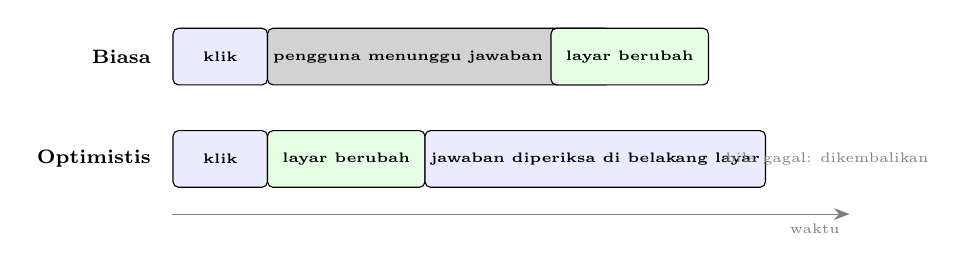
\begin{tikzpicture}[
    font=\scriptsize,
    langkah/.style={draw, rounded corners=2pt, minimum height=0.72cm,
                    align=center, anchor=west, font=\tiny\bfseries,
                    inner xsep=2pt},
    baris/.style={anchor=east, font=\scriptsize\bfseries}
  ]
    \node[baris] at (-0.15,0) {Biasa};
    \node[langkah, minimum width=1.2cm, fill=blue!8] at (0,0) {klik};
    \node[langkah, minimum width=3.6cm, fill=gray!35] at (1.2,0)
      {pengguna menunggu jawaban server};
    \node[langkah, minimum width=2.0cm, fill=green!10] at (4.8,0)
      {layar berubah};
    \node[baris] at (-0.15,-1.3) {Optimistis};
    \node[langkah, minimum width=1.2cm, fill=blue!8] at (0,-1.3) {klik};
    \node[langkah, minimum width=2.0cm, fill=green!10] at (1.2,-1.3)
      {layar berubah};
    \node[langkah, minimum width=3.6cm, fill=blue!8] at (3.2,-1.3)
      {jawaban diperiksa di belakang layar};
    \node[anchor=west, font=\tiny, gray] at (6.9,-1.3)
      {bila gagal: dikembalikan};
    \draw[-{Stealth[length=2mm]}, gray] (0,-2.0) -- (8.6,-2.0)
      node[anchor=north east, font=\tiny] {waktu};
  \end{tikzpicture}}

  \vspace{10pt}
  {\footnotesize \textit{Optimistic update} memindahkan penantian pengguna ke
  belakang layar.}
\end{frame}

\begin{frame}[fragile]{{\Large Tombol Suka: Layar Berubah Dulu}}
  \vspace{2pt}
\begin{lstlisting}[language=TypeScript]
async function tekanSuka(
  idBuku: number,
  sebelum: KeadaanSuka,
  gambarUlang: Penggambar,
): Promise<KeadaanSuka> {
  const sesudah = keadaanSesudahKlik(sebelum);
  gambarUlang(sesudah); // Pengguna melihat hasilnya sebelum server menjawab.
  try {
    const jawaban = await fetch(`${ALAMAT_SUKA}/${idBuku}`, {
      method: sesudah.sudahSuka ? "PUT" : "DELETE",
    });
    if (!jawaban.ok) {
      throw new Error(`server menolak dengan status ${jawaban.status}`);
    }
\end{lstlisting}
\end{frame}

\begin{frame}[fragile]{{\Large Tombol Suka: Dikembalikan Bila Gagal}}
  \vspace{4pt}
\begin{lstlisting}[language=TypeScript]
  } catch {
    // Dikembalikan ke keadaan sebelum klik. Tombolnya tampak "memantul".
    gambarUlang(sebelum);
    return sebelum;
  }
  const tersimpan = { ...sesudah, sedangMenyimpan: false };
  gambarUlang(tersimpan);
  return tersimpan;
}
\end{lstlisting}

  \vspace{4pt}
  {\footnotesize \texttt{PUT} dan \texttt{DELETE} dipilih karena keduanya
  idempoten, yaitu aman diulang tanpa mengubah hasil akhir. Tersedia di
  \texttt{sources/chapter04/optimistic-update.ts}.}
\end{frame}

\begin{frame}{{\Large Dua Contoh Kasus}}
  \vspace{8pt}
  \begin{enumerate}
    \item Server di Frankfurt, dengan RTT dari Jakarta sekitar 190 milidetik.
          Dengan cara biasa, tombol suka baru berubah paling cepat 190
          milidetik setelah diklik. Dengan \textit{optimistic update}, tombol
          berubah pada penggambaran layar berikutnya.
    \item Buku ditambahkan ke keranjang, lalu server menolak karena stok
          habis. Buku itu hilang lagi dari keranjang, disertai pesan
          penjelasan.
  \end{enumerate}
  \vspace{6pt}
  {\footnotesize Cocok bila kegagalan jarang dan pembatalannya tidak merugikan.
  Tidak cocok untuk pembayaran.}
\end{frame}

\begin{frame}{{\Large Dua Arti Optimistis}}
  \vspace{6pt}
  \centering
  {\small
  \begin{tabularx}{\textwidth}{lYY}
    \hline
     & \textbf{\textit{Optimistic update}} & \textbf{\textit{Optimistic locking}} \\
    \hline
    Letaknya & Antarmuka di browser & Basis data di server \\
    \hline
    Yang dianggap & Permintaan akan berhasil & Tidak ada penulis lain yang mengubah baris yang sama \\
    \hline
    Bila anggapannya salah & Tampilan dikembalikan ke keadaan sebelum klik & Penulisan ditolak, lalu diulang dari awal \\
    \hline
    Tujuannya & Pengguna tidak menunggu jawaban server & Tidak ada gembok yang ditahan selama transaksi \\
    \hline
  \end{tabularx}}
\end{frame}

\begin{frame}{{\Large Eventual Consistency}}
  \vspace{10pt}
  \begin{itemize}
    \item Salinan di browser, CDN, dan Redis tidak berubah pada saat yang sama
          ketika data diubah.
    \item Bila tidak ada perubahan baru, semua salinan pada akhirnya kembali
          sama.
    \item Kata ``pada akhirnya'' tidak menyebut berapa lama.
  \end{itemize}
  \vspace{8pt}
  {\footnotesize Analoginya pengumuman pindah ruang kuliah yang ditempel di
  beberapa gedung satu per satu. Untuk sementara, ada gedung yang masih
  memasang pengumuman lama.}
\end{frame}

\begin{frame}{{\Large Dua Jaminan bagi Pengguna}}
  \vspace{4pt}
  \centering
  {\scriptsize
  \begin{tabularx}{\textwidth}{lYY}
    \hline
    \textbf{Jaminan} & \textbf{Pelanggarannya terlihat sebagai} & \textbf{Cara menjaganya} \\
    \hline
    \textit{Read-your-writes} & Pengguna mengganti nama, lalu halaman profilnya masih menampilkan nama lama. & Hapus kunci \textit{cache} saat menulis, dan layani pengguna itu dari sumber utama selama beberapa detik sesudahnya. \\
    \hline
    \textit{Monotonic reads} & Komentar baru muncul, lalu hilang lagi setelah halaman dimuat ulang. & Arahkan pengguna yang sama ke salinan yang sama, atau kirim nomor versi terakhir yang pernah dilihatnya. \\
    \hline
  \end{tabularx}}

  \vspace{8pt}
  {\footnotesize Halaman profil yang disimpan CDN dengan \texttt{s-maxage=60}:
  pengunjung lain boleh melihat nama lama sampai 60 detik, tetapi pemilik
  profil harus langsung melihat nama barunya. Profil milik sendiri dikirim
  dengan \texttt{private, no-cache}.}
\end{frame}

\section{Timeout, Retry, dan Circuit Breaker}

\begin{frame}{\hfill}
  \centering
  \Huge{\textbf{Timeout, Retry,\\dan Circuit Breaker}}
\end{frame}

\begin{frame}{{\Large Gagal Cepat dan Gagal Lambat}}
  \vspace{10pt}
  \begin{itemize}
    \item Panggilan ke layanan lain dapat gagal dengan cepat, misalnya koneksi
          ditolak, atau gagal dengan lambat, yaitu tidak dijawab sama sekali.
    \item Kegagalan lambat lebih berbahaya. Setiap permintaan yang menunggu
          menahan satu \textit{worker}.
    \item Ketika semua \textit{worker} menunggu, aplikasi berhenti melayani, termasuk
          halaman yang tidak memerlukan layanan yang lambat itu.
  \end{itemize}
  \vspace{8pt}
  {\footnotesize Analoginya menelepon bagian keuangan kampus: tutup setelah
  sepuluh dering, telepon lagi nanti dengan jeda berbeda dari teman, dan
  berhenti menelepon sejam bila sepanjang pagi tidak diangkat.}
\end{frame}

\begin{frame}{{\Large Cara Mengukurnya}}
  \vspace{10pt}
  \begin{itemize}
    \item \texttt{layanan-lambat.py}: layanan biaya kirim tiruan yang biasanya
          menjawab dalam 20 milidetik, tetapi sebagian jawabannya ditahan 2
          detik.
    \item \texttt{resilience.py}: 10 \textit{worker} bersama-sama mengirim 100
          permintaan, dengan empat cara.
    \item Empat caranya: tanpa batas waktu, batas waktu 300 milidetik, batas
          waktu ditambah \textit{retry} sampai tiga percobaan, dan semua itu
          ditambah \textit{circuit breaker}.
  \end{itemize}
  \vspace{8pt}
  {\footnotesize Kedua berkas hanya dijalankan terhadap layanan milik
  sendiri.}
\end{frame}

\begin{frame}{{\Large Layanan Sesekali Lambat}}
  \vspace{4pt}
  \centering
  {\small
  \begin{tabularx}{\textwidth}{Xrrrrr}
    \hline
    \textbf{Cara} & \textbf{Berhasil} & \textbf{p50} & \textbf{p95} & \textbf{Panggilan} & \textbf{Durasi (s)} \\
    \hline
    \texttt{tanpa\_batas\_waktu} & 100\% & 22,1 & 2.002,3 & 100 & 4,5 \\
    \hline
    \texttt{batas\_waktu} & 82\% & 22,2 & 301,4 & 100 & 0,9 \\
    \hline
    \texttt{batas\_waktu\_retry} & 100\% & 22,1 & 371,3 & 123 & 1,3 \\
    \hline
    \texttt{circuit\_breaker} & 100\% & 22,2 & 366,5 & 121 & 1,1 \\
    \hline
  \end{tabularx}}

  \vspace{6pt}
  {\footnotesize 20 persen jawaban ditahan 2 detik, waktu dalam milidetik.
  Tanpa batas waktu, p95-nya 2.002,3 milidetik. Dengan batas waktu, p95 turun
  menjadi 301,4 milidetik, dengan harga 18 permintaan yang menyerah.
  \textit{Retry} mengembalikan keberhasilan ke 100 persen dengan 123
  panggilan.}
\end{frame}

\begin{frame}{{\Large Layanan Seluruhnya Lambat}}
  \vspace{4pt}
  \centering
  {\small
  \begin{tabularx}{\textwidth}{Xrrrrr}
    \hline
    \textbf{Cara} & \textbf{Berhasil} & \textbf{p50} & \textbf{p95} & \textbf{Panggilan} & \textbf{Durasi (s)} \\
    \hline
    \texttt{tanpa\_batas\_waktu} & 100\% & 2.002,7 & 2.004,1 & 100 & 20,0 \\
    \hline
    \texttt{batas\_waktu} & 0\% & 302,0 & 304,0 & 100 & 3,0 \\
    \hline
    \texttt{batas\_waktu\_retry} & 0\% & 973,6 & 1.032,8 & 300 & 9,9 \\
    \hline
    \texttt{circuit\_breaker} & 0\% & 0,0 & 318,8 & 10 & 0,4 \\
    \hline
  \end{tabularx}}

  \vspace{6pt}
  {\footnotesize Semua jawaban ditahan 2 detik, yaitu keadaan layanan yang
  sedang kewalahan. Waktu dalam milidetik.}
\end{frame}

\begin{frame}{{\Large Membaca Tabel Kedua}}
  \vspace{10pt}
  \begin{itemize}
    \item Tanpa batas waktu, semuanya berhasil, tetapi 10 \textit{worker} hanya mampu
          menyelesaikan 5 permintaan per detik, sehingga 100 permintaan
          memakan 20 detik.
    \item \textit{Retry} membuat layanan yang sudah kewalahan menerima 300
          panggilan, tiga kali lipat bebannya, dan tidak satu pun berhasil.
    \item \textit{Circuit breaker} hanya meneruskan 10 panggilan. Sisanya langsung
          ditolak dengan p50 0,0 milidetik, dan semuanya selesai dalam 0,4
          detik.
  \end{itemize}
\end{frame}

\begin{frame}{{\Large Mengapa 10 Panggilan, Bukan 5}}
  \vspace{10pt}
  \begin{itemize}
    \item Ambang \textit{circuit breaker} adalah lima kegagalan beruntun.
    \item Kesepuluh \textit{worker} mulai bersamaan, sehingga panggilan pertama mereka
          sudah terkirim sebelum kegagalan kelima tercatat.
    \item Panggilan uji \textit{half-open} tidak pernah terjadi, karena seluruh
          percobaan selesai dalam 0,4 detik, sebelum \textit{cooldown} satu detik
          habis.
  \end{itemize}
\end{frame}

\begin{frame}{{\Large Tiga Keadaan Circuit Breaker}}
  \vspace{8pt}
  \centering
  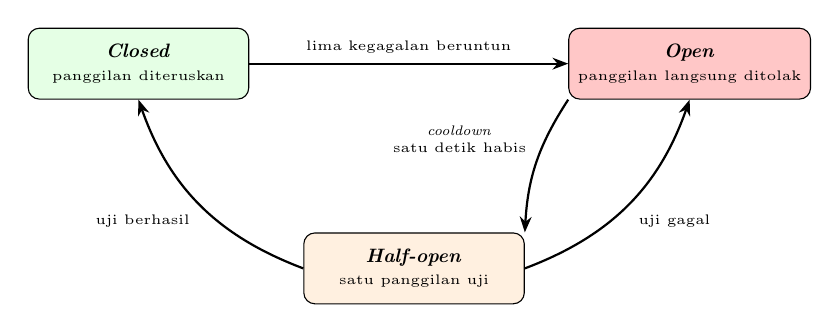
\begin{tikzpicture}[
    font=\scriptsize,
    keadaan/.style={draw, rounded corners, align=center, minimum height=0.9cm,
                    minimum width=2.8cm, font=\scriptsize\bfseries},
    panah/.style={-{Stealth[length=2mm]}, thick},
    ket/.style={font=\tiny, align=center}
  ]
    \node[keadaan, fill=green!10] (tutup) at (0,0)
      {\textit{Closed}\\{\tiny\mdseries panggilan diteruskan}};
    \node[keadaan, fill=red!22] (buka) at (7,0)
      {\textit{Open}\\{\tiny\mdseries panggilan langsung ditolak}};
    \node[keadaan, fill=orange!12] (setengah) at (3.5,-2.6)
      {\textit{Half-open}\\{\tiny\mdseries satu panggilan uji}};
    \draw[panah] (tutup) -- node[ket, above] {lima kegagalan beruntun} (buka);
    \draw[panah] (buka.south west) to[bend right=15]
      node[ket, above left] {\textit{cooldown}\\satu detik habis} (setengah.north east);
    \draw[panah] (setengah.east) to[bend right=25]
      node[ket, below right] {uji gagal} (buka.south);
    \draw[panah] (setengah.west) to[bend left=25]
      node[ket, below left] {uji berhasil} (tutup.south);
  \end{tikzpicture}
\end{frame}

\begin{frame}[fragile]{{\Large Keputusan Sebelum Tiap Panggilan}}
  \vspace{4pt}
\begin{lstlisting}[style=PythonStyle]
  def izinkan_panggilan(self):
    """Menentukan apakah satu panggilan boleh diteruskan ke layanan."""
    with self.gembok:
      if self.keadaan == CLOSED:
        return True
      cooldown_habis = time.monotonic() - self.waktu_dibuka >= COOLDOWN_DETIK
      if self.keadaan == OPEN and cooldown_habis:
        # Hanya satu panggilan uji. Sisanya ditolak sampai hasilnya ada.
        self.keadaan = HALF_OPEN
        return True
      return False
\end{lstlisting}

  \vspace{4pt}
  {\footnotesize Tersedia di \texttt{sources/chapter04/resilience.py}.}
\end{frame}

\begin{frame}[fragile]{{\Large Exponential Backoff dan Jitter}}
  \vspace{4pt}
\begin{lstlisting}[style=PythonStyle]
def hitung_jeda_sebelum_retry(percobaan_ke, pengacak):
  """Jeda acak antara nol dan batas atas yang berlipat dua tiap percobaan.

  Cara ini disebut exponential backoff dengan jitter. Tanpa unsur acak,
  seluruh klien yang gagal bersamaan akan retry bersamaan pula, dan layanan
  dihantam gelombang yang sama berulang kali.
  """
  batas_atas = min(JEDA_MAKSIMUM_DETIK, JEDA_DASAR_DETIK * 2 ** percobaan_ke)
  return pengacak.uniform(0, batas_atas)
\end{lstlisting}

  \vspace{4pt}
  {\footnotesize Makin panjang agar layanan diberi waktu pulih, acak agar
  klien yang gagal bersamaan tidak melakukan \textit{retry} bersamaan. Jeda
  pertama acak antara 0 dan 50 milidetik, jeda kedua antara 0 dan 100
  milidetik.}
\end{frame}

\begin{frame}{{\Large Aturan Retry}}
  \vspace{10pt}
  \begin{itemize}
    \item Hanya untuk permintaan idempoten. \texttt{GET}, \texttt{PUT}, dan
          \texttt{DELETE} idempoten, sedangkan \texttt{POST} tidak.
    \item \textit{Retry} pada \texttt{POST} pembayaran yang jawabannya hilang dapat
          menagih pembeli dua kali. Cara menanganinya dibahas pada Bab 12.
    \item \textit{Retry} berlipat antarlapisan: tiga lapisan yang masing-masing
          mencoba tiga kali menjadi 3 $\times$ 3 $\times$ 3 = 27 panggilan.
          Pasang di satu lapisan saja.
  \end{itemize}
\end{frame}

\begin{frame}[fragile]{{\Large Retry Tersembunyi}}
  \vspace{2pt}
\begin{lstlisting}[language=bash]
docker compose pause cache
python redis-macet.py
docker compose unpause cache

# Keluarannya:
# Satu GET ke Redis yang dibekukan, batas waktu 0.05 detik, 5 ulangan
#
#   Pengaturan          Tercepat    Tengah   Terlama  Error
#   bawaan pustaka         3.71s     4.96s     5.23s  TimeoutError
#   tanpa retry            0.05s     0.05s     0.05s  TimeoutError
\end{lstlisting}

  \vspace{2pt}
  {\footnotesize redis-py 8.1 mencoba ulang perintah yang gagal karena batas
  waktu sampai 10 kali, dengan jeda acak yang batas atasnya berlipat dua sampai
  paling lama satu detik. Batas 50 milidetik menjadi 3,71 sampai 5,23 detik.}
\end{frame}

\begin{frame}[fragile]{{\Large Mematikan Retry Bawaan}}
  \vspace{4pt}
\begin{lstlisting}[style=PythonStyle]
  cache = redis.Redis(
      host=REDIS_HOST,
      port=REDIS_PORT,
      socket_timeout=BATAS_WAKTU_REDIS_DETIK,
      socket_connect_timeout=BATAS_WAKTU_REDIS_DETIK,
      retry=Retry(NoBackoff(), JUMLAH_RETRY_REDIS),
  )
\end{lstlisting}

  \vspace{4pt}
  {\footnotesize Batas waktu yang ditulis sendiri baru dapat dipercaya setelah
  pengaturan \textit{retry} bawaan pustakanya diperiksa. Tersedia di
  \texttt{sources/chapter04/aplikasi.py}.}
\end{frame}

\begin{frame}{{\Large Dua Pelengkap}}
  \vspace{10pt}
  \begin{enumerate}
    \item Batas waktu mengecil ke arah \textit{downstream}. Bila seluruh permintaan diberi
          batas 1 detik, panggilan biaya kirim di dalamnya diberi batas lebih
          kecil, misalnya 300 milidetik.
    \item Ketika \textit{circuit breaker} dalam keadaan \textit{open}, aplikasi tetap menjawab sesuatu: tarif
          terakhir yang tersimpan di \textit{cache}, atau pesan bahwa biaya
          kirim dihitung saat pembayaran.
  \end{enumerate}
  \vspace{8pt}
  {\footnotesize Perintah \texttt{stale-if-error} pada HTTP adalah bentuk yang
  sama untuk \textit{cache} di browser dan CDN.}
\end{frame}

\section{Penyiapan Latihan}

\begin{frame}{\hfill}
  \centering
  \Huge{\textbf{Penyiapan Latihan}}
\end{frame}

\begin{frame}[fragile]{{\Large Basis Data dan Redis}}
  \vspace{2pt}
\begin{lstlisting}[language=bash]
cd sources/chapter04
docker compose up -d
./siapkan-data.sh

# Keluarannya (dipotong):
# === 02-data-uji.sql
#     tabel     | count
# --------------+--------
#  kategori     |     20
#  pelanggan    |  20000
#  buku         |  50000
#  pesanan      | 200000
#  item_pesanan | 600000
\end{lstlisting}

  \vspace{2pt}
  {\footnotesize Basis data, Redis, dan layanan biaya kirim dijalankan di
  komputer sendiri. Permintaan ke sistem luar hanya dua, ke satu aset situs
  kampus, dan keduanya bersifat mengamati.}
\end{frame}

\begin{frame}[fragile]{{\Large Venv dan Aturan Main}}
  \vspace{2pt}
\begin{lstlisting}[language=bash]
cd sources
python3 -m venv .venv
.venv/bin/pip install "psycopg[binary,pool]" sqlalchemy redis
\end{lstlisting}

  \vspace{4pt}
  \begin{itemize}
    \item Bab ini menambahkan pustaka \texttt{redis} pada venv bersama.
    \item \texttt{stampede.py} dan \texttt{resilience.py} sengaja membebani,
          sehingga tidak boleh diarahkan ke sistem milik orang lain.
    \item Hasil tiap mahasiswa akan berbeda. Yang dilaporkan adalah pola
          perbandingannya beserta penjelasannya, bukan angka persisnya.
  \end{itemize}
\end{frame}

\section{Latihan 1: Kebijakan Cache}

\begin{frame}{\hfill}
  \centering
  \Huge{\textbf{Latihan 1\\Membaca Kebijakan Cache}}
\end{frame}

\begin{frame}{{\Large Langkah Kerja}}
  \vspace{4pt}
  \begin{enumerate}
    \item Jalankan \texttt{python aplikasi.py} pada terminal pertama.
    \item Baca header halaman dan aset aplikasi, catat \texttt{Cache-Control}
          dan \texttt{ETag}-nya.
    \item Kirim permintaan bersyarat ke halaman dengan \texttt{ETag} tersebut.
    \item Kirim satu permintaan \texttt{HEAD} ke \texttt{stylenew.css} situs
          kampus, lalu hitung masa segar tebakannya.
    \item Kirim satu permintaan bersyarat ke aset kampus yang sama.
    \item Muat ulang \texttt{http://localhost:8000/} dua kali di browser, catat
          kolom \emph{Status} dan \emph{Size}.
  \end{enumerate}
  \vspace{4pt}
  {\footnotesize Permintaan yang membawa \texttt{If-None-Match} disebut
  permintaan bersyarat.}
\end{frame}

\begin{frame}[fragile]{{\Large Membaca Header}}
  \vspace{2pt}
\begin{lstlisting}[language=bash]
curl -sI http://localhost:8000/aset/app.3f9a2c.js \
  | grep -iE "^(http|cache-control)"
curl -sI https://www.pradita.ac.id/assets/front/css/stylenew.css \
  | grep -iE "^(date|last-modified|etag)"
curl -s -o /dev/null -w "%{http_code} %{size_download} byte\n" \
  -H 'If-None-Match: "67d3dca2-965"' \
  https://www.pradita.ac.id/assets/front/css/stylenew.css

# Keluarannya:
# HTTP/1.0 200 OK
# Cache-Control: public, max-age=31536000, immutable
# date: Thu, 10 Sep 2026 08:24:59 GMT
# last-modified: Fri, 14 Mar 2025 07:37:06 GMT
# etag: "67d3dca2-965"
# 304 0 byte
\end{lstlisting}
\end{frame}

\begin{frame}{{\Large Contoh Hasil Latihan 1}}
  \vspace{6pt}
  \centering
  {\footnotesize
  \begin{tabularx}{\textwidth}{lYlll}
    \hline
    \textbf{Sumber} & \textbf{\texttt{Cache-Control}} & \textbf{Masa segar} & \textbf{Biasa} & \textbf{Bersyarat} \\
    \hline
    Halaman aplikasi & \texttt{no-cache} & 0 detik & 200, 331 byte & 304, 0 byte \\
    \hline
    Aset aplikasi & \texttt{public, max-age=31536000, immutable} & 1 tahun & 200 & tanpa \texttt{ETag} \\
    \hline
    Aset kampus & tidak ada & sekitar 54 hari & 200, 2.405 byte & 304, 0 byte \\
    \hline
  \end{tabularx}}
\end{frame}

\begin{frame}{{\Large Tanda Versi Server Kampus}}
  \vspace{10pt}
  \begin{itemize}
    \item \texttt{ETag} aset kampus, \texttt{67d3dca2-965}, tersusun dari dua
          bilangan heksadesimal.
    \item \texttt{965} sama dengan 2.405, yaitu ukuran berkasnya dalam byte.
    \item \texttt{67d3dca2} sama dengan 1.741.937.826 detik sejak 1 Januari
          1970, yaitu waktu \texttt{last-modified} berkas tersebut.
  \end{itemize}
  \vspace{8pt}
  {\footnotesize Server kampus menurunkan tanda versinya dari waktu ubah dan
  ukuran berkas, sedangkan \texttt{aplikasi.py} menurunkannya dari isi berkas.
  Masa segar tebakan bergantung pada tanggal pemeriksaan.}
\end{frame}

\begin{frame}{{\Large Lembar Isian Latihan 1}}
  \vspace{4pt}
  \centering
  {\footnotesize
  \begin{tabularx}{\textwidth}{lXlll}
    \hline
    \textbf{Sumber} & \textbf{\texttt{Cache-Control}} & \textbf{Masa segar} & \textbf{Biasa} & \textbf{Bersyarat} \\
    \hline
    Halaman aplikasi & \dots & \dots & \dots & \dots \\
    \hline
    Aset aplikasi & \dots & \dots & \dots & \dots \\
    \hline
    Aset kampus & \dots & \dots & \dots & \dots \\
    \hline
    Aset lain pilihan sendiri & \dots & \dots & \dots & \dots \\
    \hline
  \end{tabularx}}

  \vspace{6pt}
  {\footnotesize Pertanyaan: mengapa halaman selalu ditanyakan ulang sedangkan
  aset aplikasi tidak pernah, berapa byte dan berapa RTT yang dihemat jawaban
  304, dan apa isi kolom \emph{Size} untuk \texttt{app.3f9a2c.js} pada muat
  ulang kedua?}
\end{frame}

\section{Latihan 2: Cache-Aside}

\begin{frame}{\hfill}
  \centering
  \Huge{\textbf{Latihan 2\\Cache-Aside dan Cache yang Macet}}
\end{frame}

\begin{frame}{{\Large Langkah Kerja}}
  \vspace{6pt}
  \begin{enumerate}
    \item Pastikan \texttt{aplikasi.py} masih menyala, lalu kosongkan kunci
          \texttt{terlaris:30hari} di Redis.
    \item Ukur \texttt{/api/terlaris} dan \texttt{/api/terlaris-cache},
          masing-masing 50 kali.
    \item Bekukan Redis dengan \texttt{docker compose pause cache}, ukur
          \texttt{/api/terlaris-cache} 20 kali, lalu cairkan lagi dengan
          \texttt{docker compose unpause cache}.
    \item Isi lembar isian, lalu jawab tiga pertanyaan analisis.
  \end{enumerate}
\end{frame}

\begin{frame}[fragile]{{\Large Mengukur Waktu Sampai Byte Pertama}}
  \vspace{2pt}
\begin{lstlisting}[language=bash]
cd sources/chapter04
source ../.venv/bin/activate
docker compose exec -T cache redis-cli DEL terlaris:30hari
python ukur-ttfb.py http://localhost:8000/api/terlaris 50
python ukur-ttfb.py http://localhost:8000/api/terlaris-cache 50

# Keluarannya (dipotong):
# p50          :    70.44 ms
# p95          :    81.99 ms
# Terbesar     :    94.41 ms
# X-Cache      : - 50
# p50          :     0.31 ms
# p95          :     0.63 ms
# Terbesar     :    67.55 ms
# X-Cache      : MISS 1, HIT 49
\end{lstlisting}
\end{frame}

\begin{frame}{{\Large Contoh Hasil Latihan 2}}
  \vspace{6pt}
  \centering
  {\small
  \begin{tabularx}{\textwidth}{Xrrrl}
    \hline
    \textbf{Keadaan} & \textbf{p50} & \textbf{p95} & \textbf{Terbesar} & \textbf{X-Cache} \\
    \hline
    Tanpa \textit{cache} & 70,44 & 81,99 & 94,41 & tidak ada \\
    \hline
    \textit{Cache-aside} & 0,31 & 0,63 & 67,55 & MISS 1, HIT 49 \\
    \hline
    Redis dibekukan & 184,72 & 188,85 & 189,07 & MISS 20 \\
    \hline
  \end{tabularx}}

  \vspace{8pt}
  {\footnotesize Dalam milidetik. Baris ketiga tampak janggal: \textit{cache}
  yang seharusnya mempercepat justru membuat jawaban dua setengah kali lebih
  lambat, karena dua kali penantian 50 milidetik ditambah kueri yang tetap
  dijalankan.}
\end{frame}

\begin{frame}{{\Large Lembar Isian Latihan 2}}
  \vspace{6pt}
  \centering
  {\small
  \begin{tabularx}{\textwidth}{Xrrrl}
    \hline
    \textbf{Keadaan} & \textbf{p50} & \textbf{p95} & \textbf{Terbesar} & \textbf{X-Cache} \\
    \hline
    Tanpa \textit{cache} & \dots & \dots & \dots & \dots \\
    \hline
    \textit{Cache-aside} & \dots & \dots & \dots & \dots \\
    \hline
    Redis dibekukan & \dots & \dots & \dots & \dots \\
    \hline
  \end{tabularx}}

  \vspace{8pt}
  {\footnotesize Pertanyaan: mengapa nilai terbesar pada baris
  \textit{cache-aside} hampir sama dengan p50 tanpa \textit{cache}, dari mana
  angka sekitar 185 milidetik berasal, dan bagian mana dari waktu tunggu
  server situs kampus pada Bab 2 yang dapat dipangkas dengan cara ini?}
\end{frame}

\section{Latihan 3: Cache Stampede}

\begin{frame}{\hfill}
  \centering
  \Huge{\textbf{Latihan 3\\Cache Stampede}}
\end{frame}

\begin{frame}{{\Large Langkah Kerja}}
  \vspace{6pt}
  \begin{enumerate}
    \item Jalankan \texttt{stampede.py} tanpa argumen, yaitu 50 permintaan
          serentak.
    \item Catat jumlah kueri, p50, p95, dan nilai terbesar untuk ketiga cara.
    \item Ulangi dengan 10 dan 100 permintaan serentak.
    \item Jalankan sekali lagi dengan satu permintaan saja, lalu bandingkan
          baris \texttt{stale\_while\_revalidate}.
    \item Isi lembar isian, lalu jawab tiga pertanyaan analisis.
  \end{enumerate}
\end{frame}

\begin{frame}[fragile]{{\Large Menjalankan Peragaan}}
  \vspace{4pt}
\begin{lstlisting}[language=bash]
cd sources/chapter04
source ../.venv/bin/activate
python stampede.py

# Keluarannya:
# 50 permintaan serentak tepat setelah kunci kedaluwarsa
#
#   Cara                    Kueri    p50 (ms)    p95 (ms)   Maks (ms)
#   tanpa_pengaman             50       895.7      1529.3      1564.3
#   single_flight               1       137.5       143.2       143.7
#   stale_while_revalidate      1         8.8        12.6        14.0
\end{lstlisting}

  \vspace{4pt}
  {\footnotesize Skrip ini sengaja membebani basis data. Jalankan hanya pada
  container milik sendiri.}
\end{frame}

\begin{frame}{{\Large Contoh Hasil Latihan 3}}
  \vspace{6pt}
  \centering
  {\small
  \begin{tabularx}{\textwidth}{Xrrrr}
    \hline
    \textbf{Cara} & \textbf{Kueri, 50} & \textbf{p50, 50} & \textbf{p95, 50} & \textbf{p50, 1} \\
    \hline
    \texttt{tanpa\_pengaman} & 50 & 895,7 & 1.529,3 & 135,2 \\
    \hline
    \texttt{single\_flight} & 1 & 137,5 & 143,2 & 125,1 \\
    \hline
    \texttt{stale\_while\_revalidate} & 1 & 8,8 & 12,6 & 0,6 \\
    \hline
  \end{tabularx}}

  \vspace{8pt}
  {\footnotesize Angka pada judul kolom adalah jumlah permintaan serentak, waktu
  dalam milidetik. Dengan satu permintaan, nilai basi terbaca dalam 0,6
  milidetik. Dengan 50 permintaan, angka itu naik menjadi 8,8 milidetik karena
  50 utas program uji bergantian berjalan.}
\end{frame}

\begin{frame}{{\Large Lembar Isian Latihan 3}}
  \vspace{6pt}
  \centering
  {\small
  \begin{tabularx}{\textwidth}{Xrrrr}
    \hline
    \textbf{Cara} & \textbf{Kueri, 100} & \textbf{p95, 10} & \textbf{p95, 50} & \textbf{p95, 100} \\
    \hline
    \texttt{tanpa\_pengaman} & \dots & \dots & \dots & \dots \\
    \hline
    \texttt{single\_flight} & \dots & \dots & \dots & \dots \\
    \hline
    \texttt{stale\_while\_revalidate} & \dots & \dots & \dots & \dots \\
    \hline
  \end{tabularx}}

  \vspace{8pt}
  {\footnotesize Pertanyaan: mengapa p50 \texttt{tanpa\_pengaman} jauh lebih
  besar daripada satu kueri padahal kuerinya sama, mengapa \texttt{single\_flight}
  tetap satu kueri berapa pun jumlah permintaannya, dan apa yang dikorbankan
  \texttt{stale\_while\_revalidate}?}
\end{frame}

\section{Latihan 4: Data Basi}

\begin{frame}{\hfill}
  \centering
  \Huge{\textbf{Latihan 4\\Data Basi Setelah Perubahan}}
\end{frame}

\begin{frame}{{\Large Langkah Kerja}}
  \vspace{6pt}
  \begin{enumerate}
    \item Jalankan \texttt{invalidasi.py}, lalu catat jumlah pembacaan basi
          dan lama basinya untuk keempat cara.
    \item Ubah \texttt{TTL\_DETIK} menjadi 10, jalankan ulang, lalu
          bandingkan.
    \item Kembalikan \texttt{TTL\_DETIK} menjadi 5, ubah
          \texttt{JEDA\_HAPUS\_KEDUA\_DETIK} menjadi 1.0, jalankan ulang, lalu
          perhatikan baris terakhir.
    \item Isi lembar isian, lalu jawab tiga pertanyaan analisis.
  \end{enumerate}
\end{frame}

\begin{frame}[fragile]{{\Large Mengukur Lama Data Basi}}
  \vspace{4pt}
\begin{lstlisting}[language=bash]
cd sources/chapter04
source ../.venv/bin/activate
python invalidasi.py

# Keluarannya:
# Harga 50000 menjadi 55000, TTL 5 detik, dibaca tiap 0.1 detik
#
#   Cara                  Baca basi  Lama basi (s)
#   ttl_saja                     50            5.1
#   hapus_saat_menulis            0            0.0
#   hapus_kalah_race             50            5.1
#   hapus_dua_kali                5            0.5
\end{lstlisting}
\end{frame}

\begin{frame}{{\Large Contoh Hasil Latihan 4}}
  \vspace{6pt}
  \centering
  {\small
  \begin{tabularx}{\textwidth}{Xrr}
    \hline
    \textbf{Cara} & \textbf{Pembacaan basi} & \textbf{Lama basi (detik)} \\
    \hline
    \texttt{ttl\_saja} & 50 & 5,1 \\
    \hline
    \texttt{hapus\_saat\_menulis} & 0 & 0,0 \\
    \hline
    \texttt{hapus\_kalah\_race} & 50 & 5,1 \\
    \hline
    \texttt{hapus\_dua\_kali} & 5 & 0,5 \\
    \hline
  \end{tabularx}}

  \vspace{8pt}
  {\footnotesize Baris pertama dan ketiga sama persis, karena \textit{race
  condition}-nya sengaja dipaksa selalu terjadi. Pada sistem sungguhan
  \textit{race condition} itu jarang, tetapi pada lalu lintas tinggi tetap
  terjadi sesekali.}
\end{frame}

\begin{frame}{{\Large Lembar Isian Latihan 4}}
  \vspace{6pt}
  \centering
  {\small
  \begin{tabularx}{\textwidth}{Xrrr}
    \hline
    \textbf{Cara} & \textbf{TTL 5} & \textbf{TTL 10} & \textbf{TTL 5, jeda kedua 1,0} \\
    \hline
    \texttt{ttl\_saja} & \dots & \dots & \dots \\
    \hline
    \texttt{hapus\_saat\_menulis} & \dots & \dots & \dots \\
    \hline
    \texttt{hapus\_kalah\_race} & \dots & \dots & \dots \\
    \hline
    \texttt{hapus\_dua\_kali} & \dots & \dots & \dots \\
    \hline
  \end{tabularx}}

  \vspace{8pt}
  {\footnotesize Pertanyaan: mengapa \texttt{hapus\_kalah\_race} sama
  buruknya dengan \texttt{ttl\_saja}, baris mana yang berubah ketika TTL
  menjadi 10 detik, dan berapa jeda penghapusan kedua yang aman bila pembaca
  paling lambat butuh 300 milidetik?}
\end{frame}

\section{Latihan 5: Resilience}

\begin{frame}{\hfill}
  \centering
  \Huge{\textbf{Latihan 5\\Batas Waktu, Retry,\\dan Circuit Breaker}}
\end{frame}

\begin{frame}{{\Large Langkah Kerja}}
  \vspace{6pt}
  \begin{enumerate}
    \item Jalankan \texttt{python layanan-lambat.py} pada terminal kedua.
    \item Jalankan \texttt{resilience.py} pada terminal lain, lalu catat
          keempat baris pada kedua skenario.
    \item Ubah \texttt{AMBANG\_GAGAL\_BERUNTUN} menjadi 3, jalankan ulang, dan
          catat jumlah panggilan \textit{circuit breaker} pada skenario seluruhnya
          lambat.
    \item Bekukan Redis, jalankan \texttt{redis-macet.py}, lalu cairkan Redis
          kembali.
    \item Isi lembar isian, lalu jawab tiga pertanyaan analisis.
  \end{enumerate}
\end{frame}

\begin{frame}[fragile]{{\Large Menjalankan Perbandingan}}
  \vspace{4pt}
\begin{lstlisting}[language=bash]
cd sources/chapter04
source ../.venv/bin/activate
python layanan-lambat.py        # terminal kedua, biarkan menyala
python resilience.py            # terminal lain

# Keluarannya (dipotong, skenario seluruhnya lambat):
#   Cara                Berhasil  p50 (ms)  p95 (ms)  Panggilan Durasi (s)
#   tanpa_batas_waktu       100%    2002.7    2004.1        100       20.0
#   batas_waktu               0%     302.0     304.0        100        3.0
#   batas_waktu_retry         0%     973.6    1032.8        300        9.9
#   circuit_breaker           0%       0.0     318.8         10        0.4
\end{lstlisting}

  \vspace{4pt}
  {\footnotesize Skrip ini mengirim ratusan permintaan. Arahkan hanya ke
  layanan milik sendiri.}
\end{frame}

\begin{frame}{{\Large Contoh Hasil Latihan 5}}
  \vspace{6pt}
  \centering
  {\small
  \begin{tabularx}{\textwidth}{Xrrrrr}
    \hline
     & \multicolumn{2}{c}{\textbf{Sesekali lambat}} & \multicolumn{3}{c}{\textbf{Seluruhnya lambat}} \\
    \hline
    \textbf{Cara} & \textbf{Berhasil} & \textbf{Panggilan} & \textbf{Berhasil} & \textbf{Panggilan} & \textbf{Durasi (s)} \\
    \hline
    \texttt{tanpa\_batas\_waktu} & 100\% & 100 & 100\% & 100 & 20,0 \\
    \hline
    \texttt{batas\_waktu} & 82\% & 100 & 0\% & 100 & 3,0 \\
    \hline
    \texttt{batas\_waktu\_retry} & 100\% & 123 & 0\% & 300 & 9,9 \\
    \hline
    \texttt{circuit\_breaker} & 100\% & 121 & 0\% & 10 & 0,4 \\
    \hline
  \end{tabularx}}

  \vspace{8pt}
  {\footnotesize Tiga angka menyimpang dari hitungan di atas kertas: 82 persen,
  bukan 80 persen; 100 persen, sedikit di atas 99,2 persen; dan 10 panggilan
  \textit{circuit breaker} walaupun ambangnya lima.}
\end{frame}

\begin{frame}{{\Large Lembar Isian Latihan 5}}
  \vspace{4pt}
  \centering
  {\footnotesize
  \begin{tabularx}{\textwidth}{Xrrrrr}
    \hline
     & \multicolumn{2}{c}{\textbf{Sesekali lambat}} & \multicolumn{3}{c}{\textbf{Seluruhnya lambat}} \\
    \hline
    \textbf{Cara} & \textbf{Berhasil} & \textbf{Panggilan} & \textbf{Berhasil} & \textbf{Panggilan} & \textbf{Durasi (s)} \\
    \hline
    \texttt{tanpa\_batas\_waktu} & \dots & \dots & \dots & \dots & \dots \\
    \hline
    \texttt{batas\_waktu} & \dots & \dots & \dots & \dots & \dots \\
    \hline
    \texttt{batas\_waktu\_retry} & \dots & \dots & \dots & \dots & \dots \\
    \hline
    \texttt{circuit\_breaker} & \dots & \dots & \dots & \dots & \dots \\
    \hline
    \texttt{circuit\_breaker}, ambang 3 & \dots & \dots & \dots & \dots & \dots \\
    \hline
  \end{tabularx}}

  \vspace{6pt}
  {\footnotesize Pertanyaan: mengapa \texttt{tanpa\_batas\_waktu} berhasil 100
  persen tetapi tetap cara terburuk, berapa kali lipat beban akibat
  \textit{retry}, dan mengapa \texttt{redis-macet.py} butuh beberapa detik padahal
  batas waktunya 50 milidetik?}
\end{frame}

\begin{frame}{{\Large Membersihkan}}
  \vspace{12pt}
  \begin{itemize}
    \item Hentikan \texttt{aplikasi.py} dan \texttt{layanan-lambat.py} dengan
          Ctrl+C.
    \item Hentikan container dengan \texttt{docker compose down -v}.
    \item Opsi \texttt{-v} ikut menghapus volume datanya, sehingga penyiapan
          berikutnya dimulai dari keadaan bersih.
  \end{itemize}
\end{frame}

\section{Ringkasan}

\begin{frame}{\hfill}
  \centering
  \Huge{\textbf{Ringkasan}}
\end{frame}

\begin{frame}{{\Large Ringkasan}}
  \begin{itemize}
    \item Salinan segar dipakai tanpa jaringan. Jawaban 304 menghemat isi,
          tetapi tidak menghemat RTT.
    \item Tanpa kebijakan, browser menebak: aset kampus dianggap segar sekitar
          54 hari.
    \item \textit{Cache-aside} menurunkan p50 dari 70,44 menjadi 0,31
          milidetik. Redis yang macet menaikkannya menjadi 184,72 milidetik.
    \item Penghapusan yang kalah dalam \textit{race condition} bertahan 5,1
          detik. \textit{Single-flight} mengubah 50 kueri serentak menjadi satu.
    \item \textit{Retry} tanpa \textit{circuit breaker}: 300 panggilan tanpa
          satu pun berhasil. \textit{Circuit breaker}: 10 panggilan, 0,4 detik.
  \end{itemize}
  \vspace{4pt}
  {\footnotesize TTL, batas waktu, dan jumlah \textit{retry} dipilih berdasarkan
  angka pengukuran.}
\end{frame}

\end{document}
